% Informe - Proyecto Final 2 - CS2023 Algoritmos y Estructuras de Datos 2026-2
% Estructura asignada: componentes biconexas.
% Compilar con pdfLaTeX. Archivos necesarios: main.tex, logo_utec.png y la
% carpeta figuras/ (fig_ejecucion.png, fig_resultado.png, fig_casos.png,
% fig_complejidad.png).
\documentclass[11pt,a4paper]{article}

\usepackage[utf8]{inputenc}
\usepackage[T1]{fontenc}
\usepackage{lmodern}
\IfFileExists{spanish.ldf}
  {\usepackage[spanish,es-tabla,es-nodecimaldot,es-noshorthands]{babel}}
  {\usepackage{babel}\babelprovide[import,main]{spanish}}
\usepackage{microtype}

\usepackage[a4paper,top=2cm,bottom=2cm,left=2cm,right=2cm,headheight=14pt]{geometry}
\usepackage{fancyhdr}
\pagestyle{fancy}
\fancyhf{}
\fancyhead[L]{\small Algoritmos y Estructuras de Datos 2026-2 · Proyecto Final 2}
\fancyhead[R]{\small Componentes biconexas}
\fancyfoot[C]{\small Página \thepage\ de \pageref{LastPage}}
\renewcommand{\headrulewidth}{0.4pt}
\usepackage{lastpage}

\usepackage{amsmath,amssymb,mathtools}
\numberwithin{equation}{section}
\newcommand{\tin}{\mathit{tin}}
\newcommand{\low}{\mathit{low}}

\usepackage{graphicx}
\graphicspath{{figuras/}}
\usepackage{booktabs,array,tabularx}
\usepackage[table]{xcolor}
\usepackage{caption}
\captionsetup{font=small,labelfont=bf,labelsep=period,skip=4pt}
\usepackage{float}
\usepackage[section]{placeins}
\usepackage{tikz}
\usetikzlibrary{arrows.meta,positioning}
\usepackage{enumitem}
\setlist{nosep,leftmargin=*}
\usepackage{titlesec}
\titleformat{\section}{\large\bfseries\color{azulutec}}{\thesection.}{0.5em}{}
\titleformat{\subsection}{\normalsize\bfseries}{\thesubsection.}{0.5em}{}
\titlespacing*{\section}{0pt}{10pt plus 2pt minus 2pt}{4pt}
\titlespacing*{\subsection}{0pt}{6pt plus 2pt minus 1pt}{2pt}
\definecolor{azulutec}{RGB}{0,51,102}
\definecolor{grisclaro}{RGB}{242,244,248}

\usepackage[hidelinks]{hyperref}
\hypersetup{colorlinks=true,linkcolor=azulutec,urlcolor=blue!60!black,citecolor=azulutec}
\usepackage{url}
\urlstyle{same}

\AtBeginDocument{%
  \renewcommand{\tablename}{Tabla}%
  \renewcommand{\figurename}{Figura}%
  \renewcommand{\refname}{Referencias}}

\setlength{\intextsep}{7pt plus 2pt minus 2pt}
\setlength{\textfloatsep}{8pt plus 2pt minus 2pt}
\setlength{\parindent}{0pt}
\setlength{\parskip}{3pt}

% Enlaces de la entrega (REEMPLAZAR antes de compilar la version final)
\newcommand{\enlacerepo}{https://github.com/COMPLETAR/aed_componentes-biconexas}
\newcommand{\enlacevideo}{https://COMPLETAR_ENLACE_DEL_VIDEO}

\begin{document}

% ------------------------------ Carátula ------------------------------
\begin{titlepage}
\thispagestyle{empty}
\centering
\IfFileExists{logo_utec.png}
  {
\includegraphics[width=0.30\textwidth]{logo_utec.png}}
  {\fbox{\parbox[c][2.6cm][c]{0.38\textwidth}{\centering\sffamily
   [Logotipo UTEC]\\[2pt]\footnotesize subir \texttt{logo\_utec.png}}}}

\vspace{1.6cm}
{\color{azulutec}\rule{\textwidth}{1.2pt}}\\[0.5cm]
{\LARGE\bfseries Algoritmos y Estructuras de Datos 2026-2 -- Informe -- Proyecto Final 2\par}
\vspace{0.6cm}
{\Large Componentes biconexas:\\[2pt]
un recorrido en profundidad, dos números por vértice y una pila de aristas\par}
\vspace{0.3cm}
{\large\itshape Anima tu algoritmo · Estructura asignada n.º 9\par}
{\color{azulutec}\rule{\textwidth}{1.2pt}}

\vspace{2.2cm}
{\large
\begin{tabular}{>{\bfseries}r l}
Curso:    & CS2023 Algoritmos y Estructuras de Datos \\[3pt]
Profesor: & Wilder Nina Choquehuayta \\[3pt]
Sección:  & COMPLETAR \\[3pt]
\end{tabular}\par}

\vspace{1.2cm}
{\large\bfseries Integrantes\par}
\vspace{0.25cm}
{\large
\begin{tabular}{l c}
\toprule
\textbf{Apellidos y nombres} & \textbf{Código} \\
\midrule
Alca, Leonardo & COMPLETAR \\
Nieva, Luis    & COMPLETAR \\
Zheng, Enrique & COMPLETAR \\
\bottomrule
\end{tabular}\par}

\vfill
{\large Lima, noviembre de 2026\par}
\end{titlepage}

% ------------------------------ Resumen -------------------------------
\setcounter{page}{2}
\section{Resumen}
Se presenta un video educativo, al estilo de Manim, que explica cómo se obtienen las componentes biconexas y los puntos de articulación de un grafo no dirigido. El algoritmo, implementado por el grupo en C++, hace un único recorrido en profundidad (DFS) y guarda dos números por vértice: el instante de descubrimiento $\tin$ y el valor $\low$. Con ellos y una pila de aristas identifica cada componente en el momento en que el recorrido regresa de un hijo a su padre. La animación no se dibuja a mano: el programa emite un evento por cada paso real de la ejecución y Manim representa esos eventos, de modo que los valores, la pila y las componentes que aparecen en pantalla son los que produjo el código. La implementación coincide con una fuerza bruta independiente en 30\,000 grafos aleatorios, y los contadores de operaciones confirman el costo $O(|V|+|E|)$ en tiempo y memoria, frente a $O(|V|\,(|V|+|E|))$ del método ingenuo.

\medskip
\textbf{Palabras clave:} componentes biconexas, puntos de articulación, búsqueda en profundidad, valores \emph{low}, pila de aristas, block-cut tree, Manim.

% ---------------------- Introducción y objetivos ----------------------
\section{Introducción y objetivos}
\label{sec:intro}
Una red, sea de computadoras, eléctrica o de transporte, puede representarse como un grafo no dirigido en el que los vértices son los nodos de la red y las aristas, sus enlaces. Una pregunta natural sobre su robustez es qué ocurre cuando un único nodo deja de funcionar. Si al quitar un vértice el grafo se divide en más partes de las que tenía, ese vértice es un \emph{punto de articulación}: un punto único de falla. Las \emph{componentes biconexas} son, en cambio, las zonas del grafo que no tienen esa debilidad, es decir, las partes que siguen conectadas aunque se elimine cualquiera de sus vértices.

La forma directa de encontrarlas consiste en quitar cada vértice y volver a recorrer el grafo, lo que cuesta un recorrido completo por vértice. Hopcroft y Tarjan (1973) mostraron que basta un solo DFS si se registra, para cada vértice, hasta dónde puede ``subir'' su subárbol mediante aristas de retroceso. Esa idea es la que se explica y se anima en este proyecto.

\textbf{Objetivo general.} Explicar con una animación generada a partir de una implementación propia en C++ cómo se calculan las componentes biconexas de un grafo no dirigido en tiempo lineal.

\textbf{Objetivos específicos.}
\begin{enumerate}[label=\textbf{OE\arabic*.},leftmargin=3.2em]
\item Implementar el algoritmo sin recurrir a librerías que ya lo resuelvan y comprobar que sus resultados son correctos.
\item Hacer que la animación dependa de la ejecución real del programa y no de pasos escritos a mano.
\item Mostrar la ejecución sobre una instancia ilustrativa y sobre casos borde relevantes.
\item Justificar la complejidad temporal y espacial, y contrastarla con el método ingenuo.
\end{enumerate}

% ---------------------- Descripción del algoritmo ---------------------
\section{Descripción del algoritmo}
\label{sec:algoritmo}
\textbf{Definiciones.} Sea $G=(V,E)$ un grafo no dirigido. Un vértice es un punto de articulación si al eliminarlo aumenta el número de componentes conexas de $G$. Una componente biconexa (o bloque) es un subgrafo conexo maximal sin puntos de articulación propios. De forma equivalente, dos aristas pertenecen a la misma componente si y solo si existe un ciclo simple que pasa por ambas; por eso, en una componente con al menos tres vértices, dos vértices cualesquiera están unidos por dos caminos que no comparten vértices intermedios. Una arista que no pertenece a ningún ciclo, es decir, un puente, forma una componente por sí sola.

De la definición se sigue una propiedad que guía todo el algoritmo: las componentes biconexas \emph{particionan las aristas}, no los vértices. Cada arista pertenece a exactamente una componente, mientras que un punto de articulación pertenece a todas las componentes que se unen en él.

\textbf{Tiempos de descubrimiento y valores \emph{low}.} Durante el DFS, cada arista del grafo resulta ser una \emph{arista de árbol}, si lleva a un vértice que aún no se había visitado, o una \emph{arista de retroceso}, si llega a un ancestro ya visitado. Para cada vértice $u$ se guardan dos números:
\begin{itemize}
\item $\tin[u]$: el instante en que el DFS descubre a $u$.
\item $\low[u]$: el menor $\tin$ alcanzable desde el subárbol de $u$ usando, a lo más, una arista de retroceso.
\end{itemize}
El valor $\low$ se calcula durante el mismo recorrido con la recurrencia
\begin{equation}
\low[u]=\min\Bigl(\tin[u],\ \min_{(u,w)\ \text{de retroceso}}\tin[w],\ \min_{v\ \text{hijo de}\ u}\low[v]\Bigr).
\label{eq:low}
\end{equation}

\textbf{Condición de cierre.} Cuando el DFS termina con un hijo $v$ y regresa a su padre $u$, se evalúa
\begin{equation}
\low[v]\ \ge\ \tin[u].
\label{eq:condicion}
\end{equation}
Si se cumple, ningún vértice del subárbol de $v$ tiene una arista hacia un ancestro propio de $u$: la única salida de ese subárbol es $u$. En consecuencia, $u$ separa al subárbol de $v$ del resto del grafo y las aristas recorridas desde que se bajó por $(u,v)$ forman una componente biconexa.

\textbf{Pila de aristas.} Para recuperar esas aristas, cada arista se apila en el momento en que se recorre, sea de árbol o de retroceso. Cuando se cumple \eqref{eq:condicion}, se desapila hasta retirar la arista $(u,v)$, y lo retirado es una componente. Se apilan aristas y no vértices precisamente porque un punto de articulación pertenece a varias componentes, mientras que una arista pertenece a una sola.

\textbf{La raíz del DFS.} Para la raíz $r$, la condición \eqref{eq:condicion} se cumple siempre, pues $\tin[r]$ es el menor de todos. Sigue sirviendo para delimitar componentes, pero no para decidir si $r$ es punto de articulación. La regla correcta es otra: la raíz es punto de articulación si y solo si tiene más de un hijo en el árbol del DFS, ya que entonces no existe ninguna arista que una dos de sus subárboles.

\textbf{Esquema del algoritmo.} El siguiente esquema resume la función \texttt{dfsBiconexas} de la implementación:

{\small
\begin{verbatim}
dfs(u, padre):
    tin[u] = low[u] = temporizador++
    para cada vecino v de u, con v distinto de padre:
        si v no ha sido visitado:                    (arista de arbol)
            apilar (u, v)
            dfs(v, u)
            low[u] = min(low[u], low[v])
            si low[v] >= tin[u]:
                si u no es la raiz: u es punto de articulacion
                desapilar hasta retirar (u, v): eso es una componente
        si no, si tin[v] < tin[u]:                   (arista de retroceso)
            apilar (u, v)
            low[u] = min(low[u], tin[v])
    si u es la raiz y tuvo mas de un hijo: u es punto de articulacion
\end{verbatim}
}

La comparación $\tin[v]<\tin[u]$ en la segunda rama evita apilar dos veces una misma arista de retroceso: desde el ancestro, esa arista se ve hacia un descendiente ya visitado y se ignora.

\textbf{Usos.} Además de localizar puntos únicos de falla y de servir para diseñar redes tolerantes a fallos, las componentes biconexas son la base del \emph{block-cut tree}: un árbol que tiene un nodo por cada componente y uno por cada punto de articulación, y que une cada componente con las articulaciones que contiene. Ese árbol resume por dónde puede desconectarse el grafo y permite responder consultas de conectividad sobre una estructura mucho más simple.

% --------------------- Implementación y animación ---------------------
\section{Implementación y animación}
\label{sec:implementacion}
\textbf{Implementación en C++.} El archivo \texttt{grafo\_biconexas.cpp} contiene la clase \texttt{Grafo}, con el grafo guardado como listas de adyacencia, y el algoritmo en los métodos \texttt{dfsBiconexas} y \texttt{calcularBiconexas}. Los resultados quedan en \texttt{esArticulacion}, un arreglo booleano por vértice, y en \texttt{componentesBiconexas}, donde cada componente es la lista de sus aristas. La estructura asignada es el algoritmo de componentes biconexas, y este se programó desde cero; la pila auxiliar es \texttt{std::stack}.

\textbf{De la ejecución a la animación.} El enunciado exige que la animación esté impulsada por la implementación. Para lograrlo, el DFS llama a un conjunto de funciones \texttt{registrar...} que no intervienen en el algoritmo: cuentan operaciones y, cuando el programa se ejecuta con la opción \texttt{-{}-traza}, escriben una línea JSON por cada paso. El guion de Manim compila y ejecuta el programa, lee esas líneas y dibuja cada una (Figura~\ref{fig:flujo}). Los valores de $\tin$ y $\low$, el contenido de la pila, el color de cada componente y los puntos de articulación que se ven en el video son, por tanto, los que produjo el código. El panel de código del video también se lee del archivo fuente, y la línea resaltada es la que originó el evento que se está mostrando.

\begin{figure}[H]
\centering
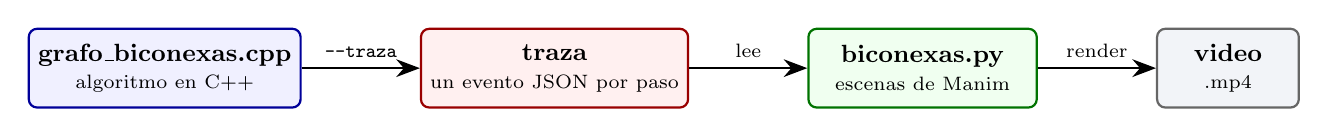
\begin{tikzpicture}[node distance=1.5cm,
  box/.style={draw,thick,rounded corners=3pt,minimum width=2.9cm,minimum height=1.0cm,align=center,font=\small},
  arr/.style={-{Stealth[length=3mm]},thick}]
\node[box,draw=blue!60!black,fill=blue!6] (cpp) {\textbf{grafo\_biconexas.cpp}\\[-1pt]{\scriptsize algoritmo en C++}};
\node[box,draw=red!60!black,fill=red!6,right=of cpp] (traza) {\textbf{traza}\\[-1pt]{\scriptsize un evento JSON por paso}};
\node[box,draw=green!45!black,fill=green!6,right=of traza] (manim) {\textbf{biconexas.py}\\[-1pt]{\scriptsize escenas de Manim}};
\node[box,draw=black!60,fill=grisclaro,right=of manim,minimum width=1.8cm] (video) {\textbf{video}\\[-1pt]{\scriptsize .mp4}};
\draw[arr] (cpp) -- node[above,font=\scriptsize]{\texttt{-{}-traza}} (traza);
\draw[arr] (traza) -- node[above,font=\scriptsize]{lee} (manim);
\draw[arr] (manim) -- node[above,font=\scriptsize]{render} (video);
\end{tikzpicture}
\caption{Flujo de generación del video. Las escenas no contienen pasos del algoritmo: solo dibujan los eventos que emite el programa.}
\label{fig:flujo}
\end{figure}

\begin{table}[H]
\centering
\caption{Eventos que emite el programa y cómo se representan en el video.}
\label{tab:eventos}
\small
\begin{tabular}{l l l}
\toprule
\textbf{Evento} & \textbf{Momento del algoritmo} & \textbf{En pantalla} \\
\midrule
\texttt{visitar}    & se asignan $\tin[u]$ y $\low[u]$            & el vértice se activa y aparece su etiqueta \\
\texttt{arbol}      & se apila una arista de árbol                & la arista se ilumina y entra una ficha a la pila \\
\texttt{retroceso}  & se apila una arista de retroceso            & arista punteada; baja el $\low$ del vértice \\
\texttt{retorno}    & se vuelve de $v$ a $u$ y se evalúa \eqref{eq:condicion} & se muestra la comparación y su respuesta \\
\texttt{componente} & se desapila hasta $(u,v)$                   & las fichas salen y la componente se colorea \\
\texttt{fin\_nodo}  & termina un vértice (regla de la raíz)       & se indica si la raíz es punto de articulación \\
\bottomrule
\end{tabular}
\end{table}

\textbf{Herramientas.} C++17 con g++ (MinGW-w64, distribución WinLibs 16.2) para la implementación; Python 3.12 y Manim Community 0.22.1 para la animación. El video se renderiza a $1920\times1080$ y 60 cuadros por segundo, y dura 4 minutos y 18 segundos.

\textbf{Contenido del video.} Se divide en tres partes de 85 segundos. La primera presenta el problema, los puntos de articulación, la definición de componente biconexa, sus usos y los valores $\tin$ y $\low$. La segunda muestra la ejecución completa sobre un grafo de 9 vértices y 11 aristas (Figura~\ref{fig:ejecucion}). La tercera trata la raíz del DFS, los casos borde, la complejidad y el block-cut tree.

\begin{figure}[H]
\centering
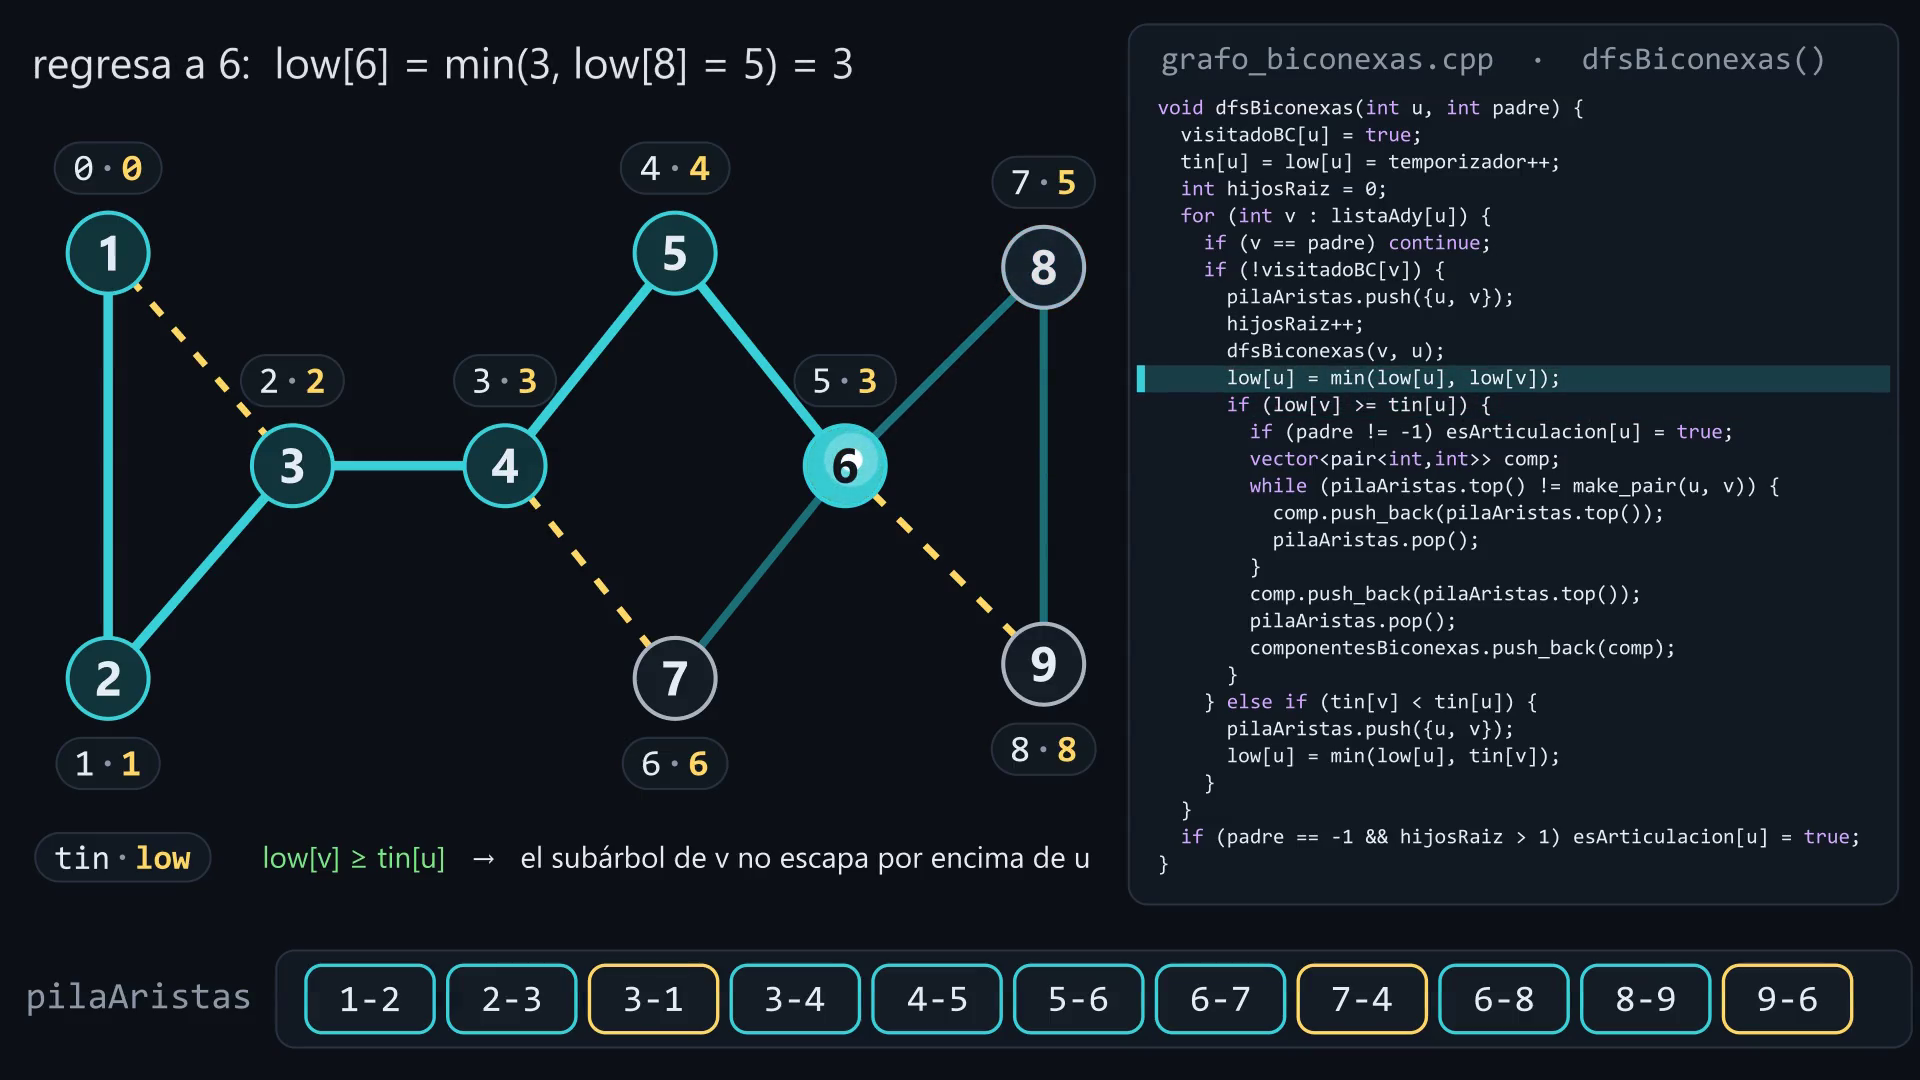
\includegraphics[width=0.49\textwidth]{fig_ejecucion.png}\hfill
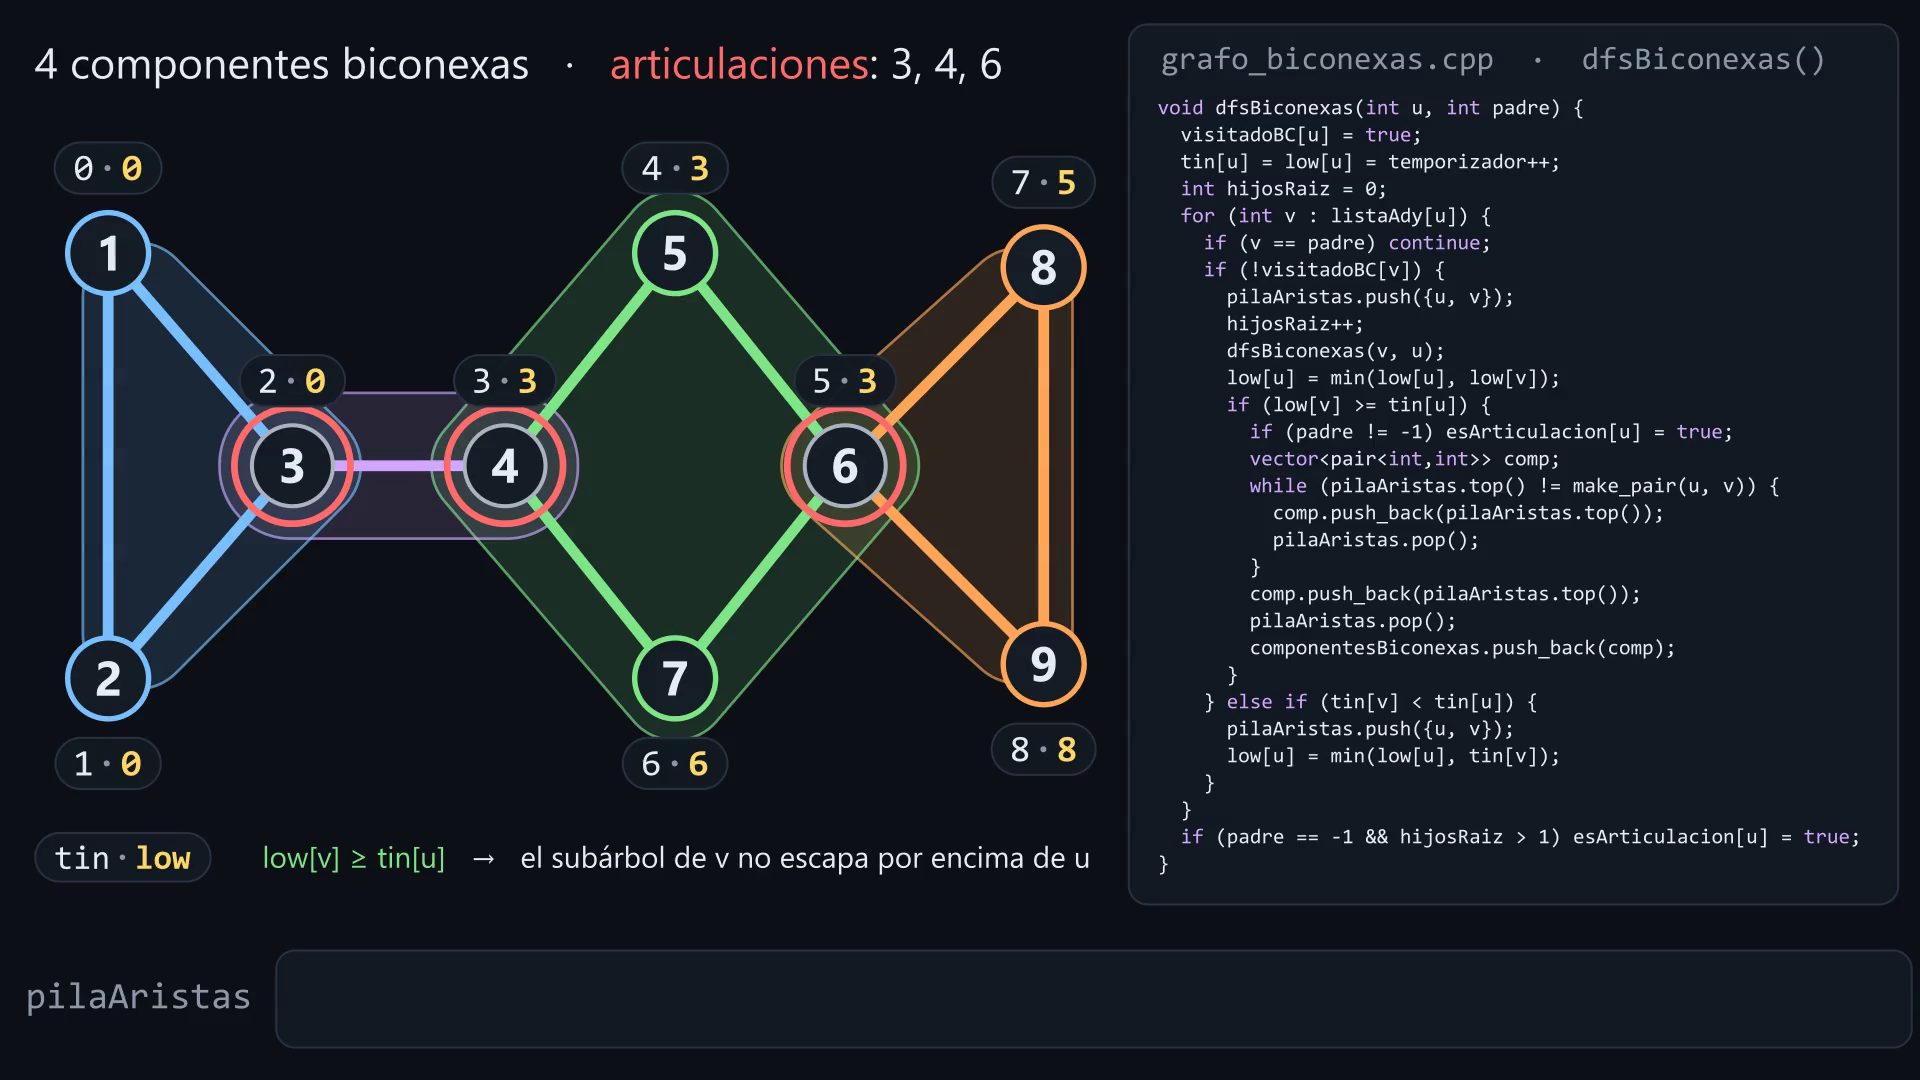
\includegraphics[width=0.49\textwidth]{fig_resultado.png}
\caption{Ejecución sobre la instancia principal. Izquierda: el DFS regresa al vértice 6 con todas las aristas apiladas; junto a cada vértice se lee $\tin\cdot\low$. Derecha: resultado final, con cuatro componentes y los puntos de articulación 3, 4 y 6.}
\label{fig:ejecucion}
\end{figure}

\textbf{Pasos para reproducir el video.} Desde la carpeta del proyecto, con g++ y Python instalados:
\begin{enumerate}[label=\arabic*.,leftmargin=2em]
\item Crear un entorno virtual: \texttt{python -m venv .venv}
\item Instalar Manim: \texttt{.venv\textbackslash Scripts\textbackslash pip install manim}
\item Generar el video: \texttt{.venv\textbackslash Scripts\textbackslash python -m manim -qh animacion/biconexas.py Video}
\end{enumerate}
El guion compila \texttt{grafo\_biconexas.cpp} si el ejecutable no existe o está desactualizado, y deja el resultado en \texttt{media/videos/biconexas/1080p60/Video.mp4}. El archivo \texttt{README.md} del proyecto detalla estos pasos y los modos adicionales del programa.

% ----------------------- Análisis de complejidad ----------------------
\section{Análisis de complejidad}
\label{sec:complejidad}
\textbf{Tiempo.} El DFS visita cada vértice una sola vez, lo que aporta $O(|V|)$. Al visitar un vértice se recorre su lista de adyacencia, y como cada arista aparece en dos listas, en total se examinan $2|E|$ entradas. Cada arista se apila exactamente una vez, como arista de árbol o como arista de retroceso vista desde el descendiente, y se desapila exactamente una vez, cuando se cierra su componente. Las demás operaciones por vértice y por arista son de tiempo constante. Por lo tanto,
\begin{equation}
T(|V|,|E|)=O(|V|)+O(2|E|)+O(|E|)+O(|E|)=O(|V|+|E|).
\label{eq:tiempo}
\end{equation}

\textbf{Memoria.} Los arreglos $\tin$, $\low$, de visitados y de articulaciones ocupan $O(|V|)$; la pila de aristas, $O(|E|)$ en el peor caso; la recursión, $O(|V|)$, y el grafo como listas de adyacencia, $O(|V|+|E|)$. El total es $O(|V|+|E|)$.

\textbf{Comprobación con contadores.} El programa cuenta estas operaciones mientras se ejecuta. En la instancia principal, con $|V|=9$ y $|E|=11$, los cuatro contadores coinciden con lo que predice el análisis (Tabla~\ref{tab:contadores}).

\begin{table}[H]
\centering
\caption{Operaciones contadas por el programa en la instancia principal ($|V|=9$, $|E|=11$).}
\label{tab:contadores}
\small
\begin{tabular}{l c c}
\toprule
\textbf{Operación} & \textbf{Valor contado} & \textbf{Valor esperado} \\
\midrule
Vértices visitados              & 9  & $|V|$ \\
Entradas de adyacencia revisadas & 22 & $2|E|$ \\
Aristas apiladas                & 11 & $|E|$ \\
Aristas desapiladas             & 11 & $|E|$ \\
\bottomrule
\end{tabular}
\end{table}

\textbf{Comparación con el método ingenuo.} El método ingenuo quita cada vértice y recuenta las componentes conexas con un recorrido completo, de modo que cuesta $O(|V|\,(|V|+|E|))$. El modo \texttt{-{}-bench} del programa cuenta las operaciones de ambos métodos sobre grafos conexos aleatorios con $|E|=2|V|$ (Tabla~\ref{tab:bench} y Figura~\ref{fig:complejidad}). Las del algoritmo crecen de forma lineal, unas nueve por vértice, mientras que las del método ingenuo crecen de forma cuadrática: con 1500 vértices la diferencia es de unas 833 veces.

\begin{table}[H]
\centering
\caption{Operaciones contadas por el modo \texttt{-{}-bench} en grafos aleatorios con $|E|=2|V|$.}
\label{tab:bench}
\small
\begin{tabular}{r r r r r}
\toprule
$|V|$ & $|E|$ & \textbf{Un solo DFS} & \textbf{Método ingenuo} & \textbf{Cociente} \\
\midrule
100  & 200  & 896     & 50\,000      & 56 \\
500  & 1000 & 4\,498  & 1\,250\,000  & 278 \\
1000 & 2000 & 8\,996  & 5\,000\,000  & 556 \\
1500 & 3000 & 13\,500 & 11\,250\,000 & 833 \\
\bottomrule
\end{tabular}
\end{table}

\begin{figure}[H]
\centering
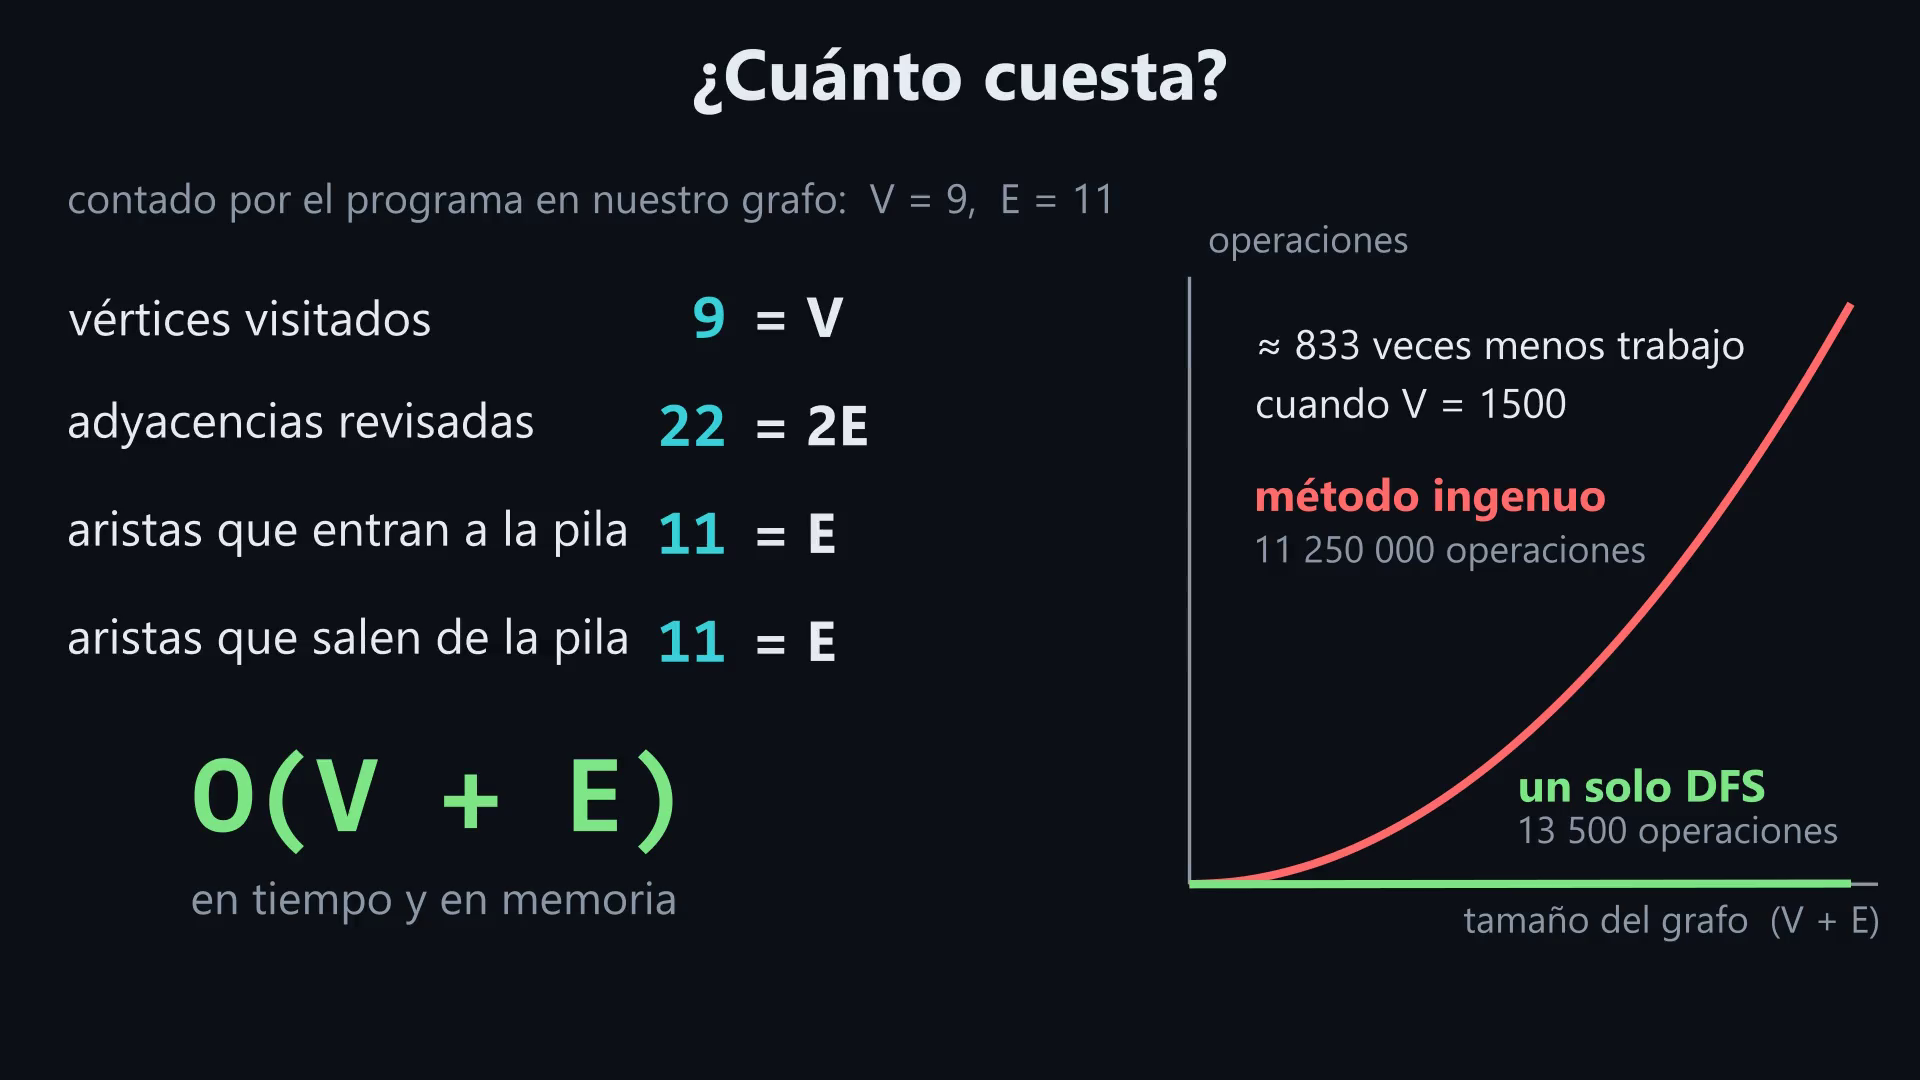
\includegraphics[width=0.72\textwidth]{fig_complejidad.png}
\caption{Escena de complejidad del video: los contadores de la instancia principal y la gráfica de operaciones del algoritmo frente al método ingenuo, ambas con datos producidos por el programa.}
\label{fig:complejidad}
\end{figure}

% -------------------- Casos borde y verificación ----------------------
\section{Casos borde y verificación}
\label{sec:casos}
\textbf{Casos borde.} El video ejecuta el mismo programa sobre cuatro situaciones límite (Figura~\ref{fig:casos}):
\begin{itemize}
\item \emph{La raíz del DFS.} En un grafo formado por dos triángulos que comparten un vértice, el recorrido empieza en ese vértice. La raíz termina con dos hijos en el árbol del DFS y el programa la marca como punto de articulación por la regla especial, no por la condición \eqref{eq:condicion}.
\item \emph{Un camino, o cualquier árbol.} No hay ciclos, así que cada arista es un puente y forma su propia componente. Con 5 vértices se obtienen 4 componentes, y los 3 vértices internos son puntos de articulación. Es el caso con más componentes posibles.
\item \emph{Un ciclo.} Todo el grafo es una sola componente y no tiene puntos de articulación.
\item \emph{Un vértice aislado.} La pila nunca recibe aristas y no se reporta ninguna componente, porque las componentes se entregan como conjuntos de aristas. Lo mismo ocurre con un grafo sin aristas.
\end{itemize}

\begin{figure}[H]
\centering
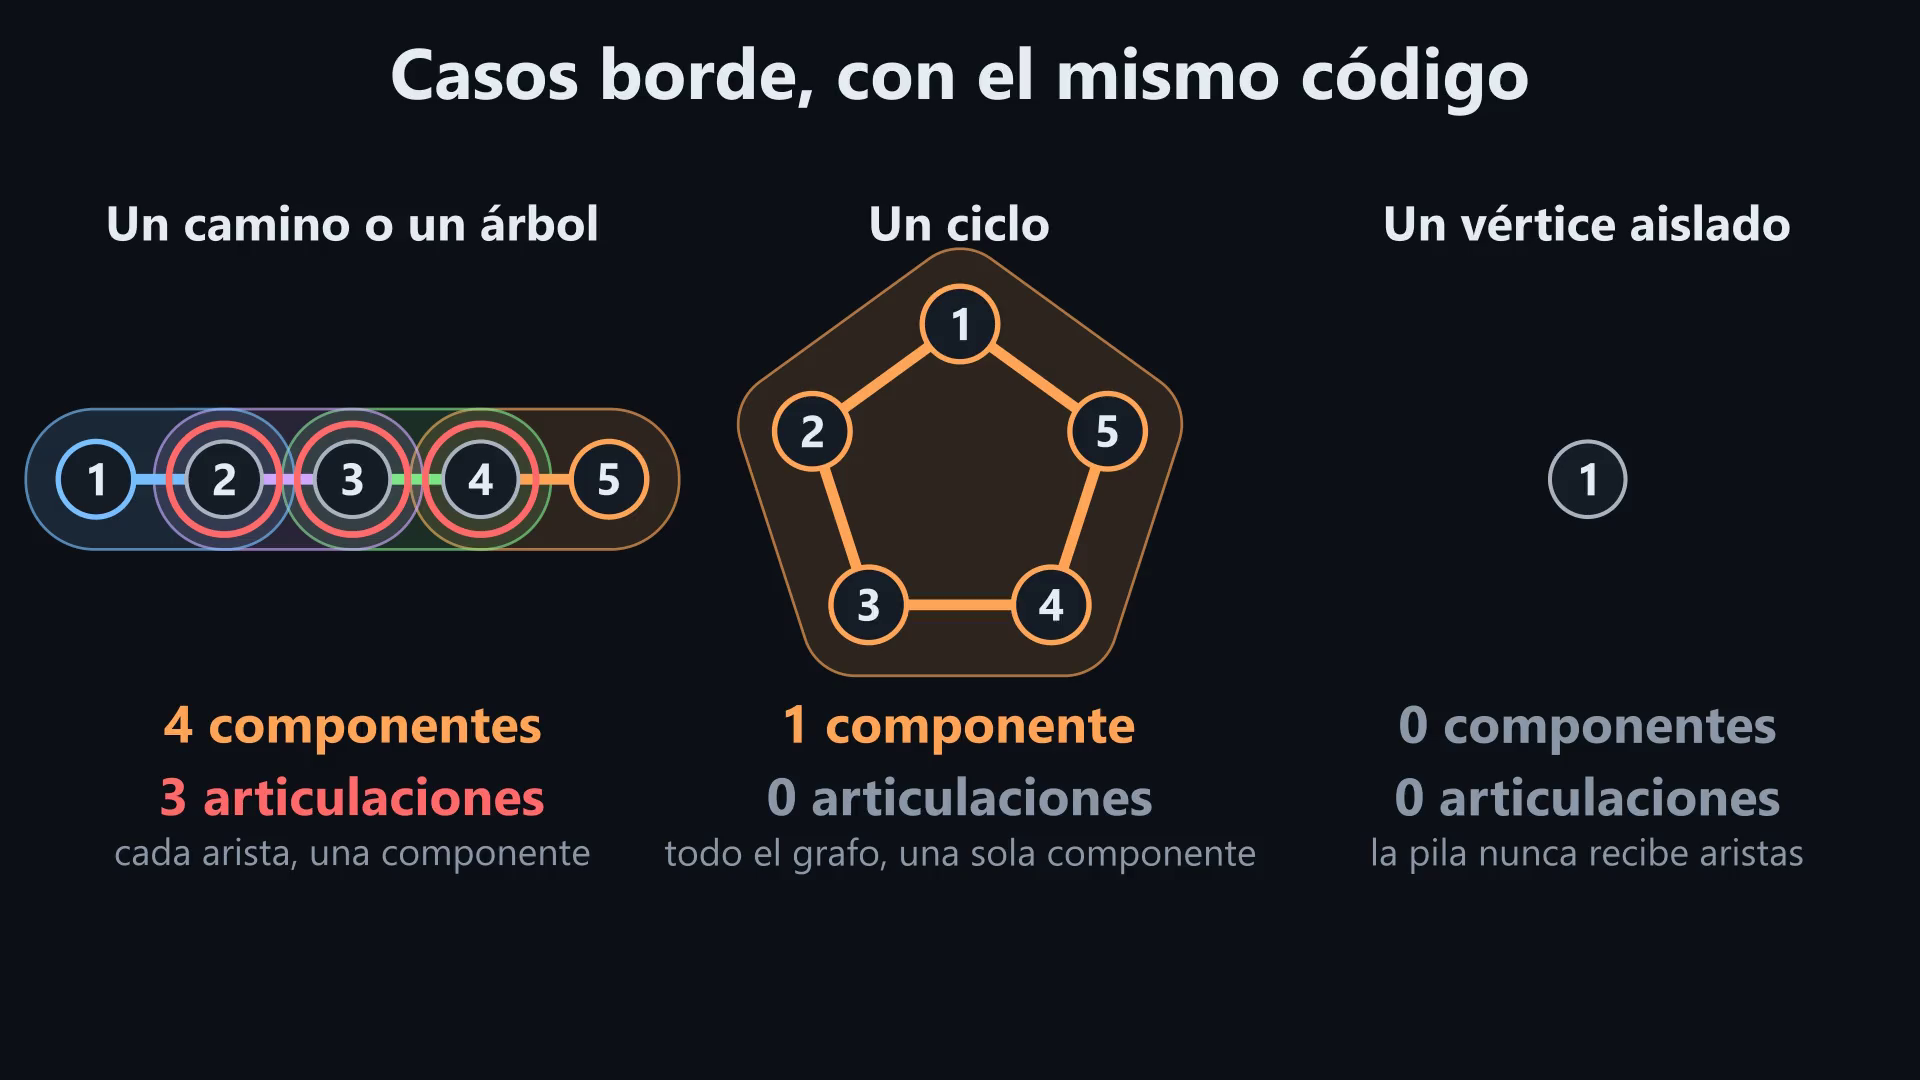
\includegraphics[width=0.72\textwidth]{fig_casos.png}
\caption{Casos borde ejecutados con la misma implementación. Los resultados que aparecen bajo cada grafo se leen de la salida del programa.}
\label{fig:casos}
\end{figure}

\textbf{Verificación.} El modo \texttt{-{}-verificar} genera grafos simples aleatorios de hasta 8 vértices y comprueba, en cada uno, que: (i) los puntos de articulación coinciden con los del método ingenuo; (ii) cada arista aparece en exactamente una componente; (iii) la partición de aristas coincide con la de una fuerza bruta independiente, que enumera todos los ciclos simples y agrupa las aristas que comparten alguno, y (iv) la pila queda vacía al terminar. Los 30\,000 grafos probados coinciden.

\textbf{Alcance.} La implementación supone grafos simples. Con aristas paralelas, los puntos de articulación siguen siendo correctos, pero la arista repetida hacia el padre no se lista dentro de su componente, porque el recorrido descarta toda arista que vuelve al padre. Al ser recursiva, en grafos muy profundos el límite práctico lo impone el tamaño de la pila de llamadas.

% ------------------------------ Evidencias ----------------------------
\section{Evidencias}
\label{sec:evidencias}
\begin{itemize}
\item \textbf{Repositorio de GitHub:} \url{\enlacerepo}
\item \textbf{Video:} \url{\enlacevideo}
\end{itemize}
Las Figuras~\ref{fig:ejecucion}, \ref{fig:complejidad} y \ref{fig:casos} son capturas del video entregado. La carpeta del proyecto contiene el código fuente del algoritmo y de la animación, las instancias de entrada, el guion narrado con sus tiempos y el archivo \texttt{README.md} con el software requerido y los pasos de compilación y ejecución.

% ---------------------------- Contribuciones --------------------------
\section{Contribuciones de cada integrante}
\label{sec:contribuciones}
\begin{table}[H]
\centering
\small
\renewcommand{\arraystretch}{2.2}
\begin{tabularx}{\textwidth}{l X}
\toprule
\textbf{Integrante} & \textbf{Contribución} \\
\midrule
Leonardo Alca  & \\
Luis Nieva     & \\
Enrique Zheng  & \\
\bottomrule
\end{tabularx}
\end{table}

% ----------------------------- Conclusiones ---------------------------
\section{Conclusiones}
\label{sec:conclusiones}
\begin{itemize}
\item Un solo recorrido en profundidad basta para obtener todas las componentes biconexas y todos los puntos de articulación. La información necesaria se reduce a dos números por vértice, y la decisión se toma con una única comparación, $\low[v]\ge\tin[u]$, cada vez que el recorrido regresa de un hijo a su padre.
\item La pila debe guardar aristas y no vértices. Las componentes biconexas particionan las aristas, mientras que un punto de articulación pertenece a varias componentes; apilar aristas es lo que permite separar cada componente sin ambigüedad.
\item La raíz del DFS necesita una regla propia. Para ella la condición general se cumple siempre, por lo que solo es punto de articulación si tiene más de un hijo en el árbol del recorrido. Este caso, junto con el árbol, el ciclo y el vértice aislado, muestra que los casos borde no requieren código adicional, pero sí entender qué reporta el algoritmo en cada uno.
\item El costo es $O(|V|+|E|)$ en tiempo y memoria. Los contadores del programa lo confirman, con $|V|$ visitas, $2|E|$ entradas de adyacencia revisadas y $|E|$ aristas apiladas y desapiladas, y la comparación con el método ingenuo muestra una diferencia de unas 833 veces con 1500 vértices.
\item Generar la animación a partir de la traza de ejecución tuvo un efecto práctico además de cumplir el enunciado: cualquier error en el algoritmo se habría visto en pantalla, y el mismo mecanismo sirvió para animar los casos borde sin escribir escenas nuevas. Como trabajo futuro se propone una versión iterativa, que evite el límite de la recursión, y el manejo de aristas paralelas.
\end{itemize}

% ----------------------------- Bibliografía ---------------------------
\section{Bibliografía}
\begingroup
\small
\begin{list}{}{\setlength{\leftmargin}{1.5em}\setlength{\itemindent}{-1.5em}\setlength{\itemsep}{2pt}\setlength{\parsep}{0pt}\setlength{\topsep}{2pt}}
\item Cormen, T. H., Leiserson, C. E., Rivest, R. L., y Stein, C. (2022). \emph{Introduction to algorithms} (4.\textsuperscript{a} ed.). MIT Press.
\item Hopcroft, J., y Tarjan, R. (1973). Algorithm 447: Efficient algorithms for graph manipulation. \emph{Communications of the ACM, 16}(6), 372--378. \url{https://doi.org/10.1145/362248.362272}
\item Sanderson, G. (s.\,f.). \emph{3Blue1Brown} [Canal de videos]. \url{https://www.3blue1brown.com/}
\item Sedgewick, R., y Wayne, K. (2011). \emph{Algorithms} (4.\textsuperscript{a} ed.). Addison-Wesley.
\item Tarjan, R. (1972). Depth-first search and linear graph algorithms. \emph{SIAM Journal on Computing, 1}(2), 146--160. \url{https://doi.org/10.1137/0201010}
\item The Manim Community Developers. (s.\,f.). \emph{Manim: Mathematical animation framework} (versión 0.22.1) [Software]. \url{https://www.manim.community/}
\end{list}
\endgroup

\end{document}
